\documentclass[10pt,twocolumn]{article}
\usepackage[margin=0.8in,top=0.9in,bottom=0.9in]{geometry}
\usepackage{amsmath,amssymb,booktabs,graphicx,microtype,xcolor,url}
\usepackage[numbers,sort&compress]{natbib}
\usepackage[hidelinks]{hyperref}
\usepackage{caption}
\captionsetup{font=small,labelfont=bf}
\renewcommand{\topfraction}{0.95}\renewcommand{\textfraction}{0.05}\renewcommand{\floatpagefraction}{0.75}
\newcommand{\nMetrics}{100}
\newcommand{\nConstant}{10}
\newcommand{\nReps}{42}
\newcommand{\nCands}{24}
\newcommand{\kSel}{3}
\newcommand{\selList}{tok\_f1, num\_decay\_2p5, bigram\_rec}
\newcommand{\nAnchors}{12,813}
\newcommand{\nOps}{20}
\newcommand{\nAnchorDatasets}{14}
\newcommand{\nModels}{4}
\newcommand{\nDatasets}{7}
\newcommand{\nPendingDatasets}{7}
\newcommand{\gridStep}{0.02}
\newcommand{\nGrid}{6,630}
\newcommand{\topK}{100}
\newcommand{\meanLambda}{0.63}
\newcommand{\meanW}{tok\_f1 0.16, num\_decay\_2p5 0.81, bigram\_rec 0.03}
\newcommand{\Jtop}{0.910}
\newcommand{\JtopHundred}{0.899}
\newcommand{\JmedGrid}{0.870}
\newcommand{\rhoEns}{0.906}
\newcommand{\aucEns}{0.997}
\newcommand{\jsEns}{0.053}
\newcommand{\badEns}{0.022}
\newcommand{\tauNatEns}{0.678}
\newcommand{\lodoRhoSel}{0.882}
\newcommand{\lodoRhoNative}{0.811}
\newcommand{\lodoRhoEm}{0.822}
\newcommand{\lodoMeanLodo}{0.895}
\newcommand{\lodoMeanFull}{0.900}
\newcommand{\lodoSameSel}{57}
\newcommand{\sevShift}{0.168}
\newcommand{\sevSelChanged}{40}
\newcommand{\probeMaeEns}{0.095}
\newcommand{\probeMaeNative}{0.145}
\newcommand{\probeMaeEm}{0.196}
\newcommand{\probeMaeF}{0.139}
\newcommand{\topOne}{claude-sonnet-5}
\newcommand{\topTwo}{gpt-5.5}
\newcommand{\tauNativePool}{0.82}
\newcommand{\pairTau}{-0.07}
\newcommand{\JNativeStyleMetric}{0.913}
\newcommand{\rhoNativeStyleMetric}{0.830}
\newcommand{\tauNatNativeStyleMetric}{0.924}
\newcommand{\badNativeStyleMetric}{0.004}
\newcommand{\JEmNorm}{0.882}
\newcommand{\rhoEmNorm}{0.848}
\newcommand{\tauNatEmNorm}{0.629}
\newcommand{\badEmNorm}{0.002}
\newcommand{\JTokFOne}{0.860}
\newcommand{\rhoTokFOne}{0.852}
\newcommand{\tauNatTokFOne}{0.544}
\newcommand{\badTokFOne}{0.006}
\newcommand{\JRougeL}{0.853}
\newcommand{\rhoRougeL}{0.858}
\newcommand{\tauNatRougeL}{0.496}
\newcommand{\badRougeL}{0.006}
\newcommand{\JNumTolOne}{0.888}
\newcommand{\rhoNumTolOne}{0.803}
\newcommand{\tauNatNumTolOne}{0.792}
\newcommand{\badNumTolOne}{0.005}
\newcommand{\JUniformOverSelectedNoGate}{0.855}
\newcommand{\rhoUniformOverSelectedNoGate}{0.893}
\newcommand{\tauNatUniformOverSelectedNoGate}{0.471}
\newcommand{\badUniformOverSelectedNoGate}{0.012}
\newcommand{\JEnsembleTopHundred}{0.903}
\newcommand{\rhoEnsembleTopHundred}{0.906}
\newcommand{\tauNatEnsembleTopHundred}{0.678}
\newcommand{\badEnsembleTopHundred}{0.022}

\title{\textbf{From 100 Answer Metrics to One Score:\\Anchor-Calibrated Metric Selection and Weight Ensembles for Cross-Dataset LLM Evaluation on Data-Matching Tasks}}
\author{Data Matchmaker Benchmark v3 \\ \small Green-agent evaluator for the AgentBeats A2A platform}
\date{}
\begin{document}
\maketitle
\begin{abstract}
Scoring free-text answers from language-model agents across heterogeneous data-matching benchmarks (record matching, table and financial-document question answering) requires one answer-level scoring rule that behaves identically on every dataset. We build a library of \nMetrics{} answer-level metrics spanning exact-match variants, numeric tolerance ladders, graded numeric error, token, character and sequence overlap, set containment, structure, length and commitment indicators. Rather than hand-picking weights, we (i) generate \nAnchors{} synthetic answers of \emph{known} utility from \nOps{} typed error operators on \nAnchorDatasets{} datasets, (ii) deduplicate the library by correlation and select the metrics that predict utility out of dataset (forward selection with leave-one-dataset-out stopping, keeping \kSel{}: \selList), (iii) grid-search the weights of the selected metrics together with a multiplicative hedge penalty over \nGrid{} candidates under an objective that combines anchor agreement, correct-vs-wrong separation, cross-dataset Jensen--Shannon consistency, a penalty on credit given to wrong answers, and fidelity to each dataset's native metric, and (iv) keep the \topK{} best weightings as an ensemble whose average is the final score and whose spread is its uncertainty. The ensemble reaches anchor Spearman \rhoEns{} and AUC \aucEns{} with wrong answers scored \badEns{}, versus \rhoNativeStyleMetric{} / \tauNatNativeStyleMetric{} for the typed native metric that wins the fidelity term by construction; leave-one-dataset-out anchor agreement is \lodoMeanLodo{} against \lodoMeanFull{} with full-data weights, and perturbing the severity scale by $\pm0.15$ moves the ensemble weights by $L_1=\sevShift$. Applied to \nModels{} commercial models on \nDatasets{} datasets with difficulty-adjusted pooling, bootstrap and per-weighting rank ranges, the method yields a single comparable leaderboard and ships as the scoring rule of an A2A judge. We state plainly that with four close models the ranks below the top are not separable, and that \nPendingDatasets{} additional data-matching datasets are wired in awaiting model predictions.
\end{abstract}

\section{Introduction}
A benchmark judge for data-matching agents must score answers that are yes/no match decisions (Abt-Buy, WDC Products, TabFact), numbers with units and scales (FinQA, TAT-QA, HiTab, TPC-DI aggregates), short spans and lists (WikiTableQuestions) and full sentences (FeTaQA). Each source dataset ships its own metric, so per-dataset scores are not on one scale and cannot be pooled. The usual fix, a composite of a few overlap metrics with hand-set weights, is arbitrary and, if the weights are tuned so that the models being ranked agree across datasets, circular.

We ask a different question: given a large library of cheap answer-level metrics, which ones carry information about answer quality, and how should they be combined so that the same quality receives the same score on every dataset? Our answer has four parts. (1) A \emph{library} of \nMetrics{} metrics (\S\ref{sec:lib}). (2) An \emph{anchor set}: for every gold answer, synthetic answers of known utility produced by typed error operators, which makes ``same quality'' observable without ranking any model (\S\ref{sec:anchors}). (3) \emph{Selection}: correlation deduplication and forward selection that keeps only metrics that predict utility on datasets they were not fitted on (\S\ref{sec:select}). (4) A \emph{grid search} over the selected metrics' weights and a hedge penalty, with the \topK{} best weightings retained as an ensemble (\S\ref{sec:grid}). The leaderboard then uses equal dataset weights on difficulty-adjusted scores, positional and Condorcet pooling, and two kinds of uncertainty (\S\ref{sec:pool}). The datasets' own metrics remain as a baseline column and as a fidelity term, not as the scoring rule (\S\ref{sec:results}).

\section{Related work}
Answer metrics: EM and token F1 \citep{rajpurkar2016squad}, ROUGE \citep{lin2004rouge}, BLEU \citep{papineni2002bleu}, BERTScore \citep{zhang2020bertscore}; dataset-specific rules in FinQA \citep{chen2021finqa}, TAT-QA \citep{zhu2021tatqa}, TabFact \citep{chen2020tabfact}, FeTaQA \citep{nan2022fetaqa}, WTQ \citep{pasupat2015wtq}. Metric meta-evaluation with severity-weighted error annotation (MQM) \citep{lommel2014mqm,freitag2021experts} and the warning that metric choice changes rankings \citep{mathur2020tangled}; our anchors are an MQM-style severity scale applied to controlled synthetic errors. Benchmark aggregation and rank pooling \citep{liang2022helm,colombo2022ranking,dwork2001rank,young1978consistent,cormack2009rrf}; uncertainty for model comparison \citep{dror2019deep}. Entity matching benchmarks (Magellan/DeepMatcher, WDC Products) and the TPC-DI integration task \citep{tpcdi2014} supply the data-matching half of the suite; the judge speaks A2A \citep{a2a2025}.

\section{Metric library}\label{sec:lib}
Every metric maps a (prediction, gold) pair to $[0,1]$; the prediction is reduced to its final answer (tag, \texttt{FINAL ANSWER:} line, or last short line, scaffolding stripped), normalised (Unicode, case, canonical numbers, punctuation, articles), and compared with the gold and its aliases (FinQA \texttt{14\%}$\equiv$\texttt{0.14464}, TAT-QA values with and without scale, list golds with per-element unit variants). Families and counts: exact-match variants (10), numeric tolerance ladder from 0.1\% to 20\% plus sign, magnitude, unit-equivalence and rounding hits (12), graded numeric error $e^{-\gamma\mathrm{RE}}$ for five $\gamma$, inverse, linear, log-ratio and sMAPE (9), token precision/recall/F$_\beta$, $n$-gram F, stemmed and content-word variants (12), character similarities and chrF (9), ROUGE/BLEU/METEOR-lite/TER/WER (10), set and containment (7), structure and format (7), length and abstention (5), commitment and consistency (4), task-specific (7), and an optional semantic family (8; embedding cosines, off by default). Numeric metrics fall back to exact match for non-numeric golds so that every metric is defined on every item. Percent equivalence is allowed only when a percent sign or a fraction in $(0,1)$ is involved, so that a hundredfold error is never free.

\section{Anchors: answers of known utility}\label{sec:anchors}
For each gold we generate one answer per applicable operator: correct answers in four styles (bare, verbose, tagged, paraphrase; utility $1$ or $0.95$), unit variants ($1$), near misses at three relative-error bands ($0.75/0.45/0.15$), digit typos ($0.2$), magnitude and sign errors ($0.05$), partial and superset spans ($0.5/0.6$), typos ($0.6$), shuffles ($0.4$), hedges and candidate lists ($0.3/0.25$), label flips, abstentions and random wrong answers ($0$). Operators are typed (numeric / boolean / short text / free-form) and seeded, giving \nAnchors{} answers on \nAnchorDatasets{} datasets, including datasets for which no model predictions exist yet. The utility scale is the only hand-set input; it is perturbed in \S\ref{sec:val}. Human correctness labels can replace the anchors through the same interface.

\section{Selection}\label{sec:select}
Of \nMetrics{} metrics, \nConstant{} are constant on this data; clustering the rest by $|\text{Spearman}|\ge 0.95$ across all anchors leaves \nReps{} representatives, of which \nCands{} pass an agreement floor (anchor $\rho>0.05$, AUC $>0.55$) and are not indicator families (structure, commitment, length), which act as constant offsets when added and are used as a gate instead. Forward selection adds the metric that most increases the leave-one-dataset-out Spearman between a non-negative least-squares combination and utility, stopping when the gain falls below $0.002$ (Table~\ref{tab:selected}). It keeps \kSel{} metrics: \selList{}, with LODO $\rho=\lodoRhoSel$ versus \lodoRhoNative{} for the typed native metric and \lodoRhoEm{} for exact match.

\section{Weight grid and ensemble}\label{sec:grid}
With $K$ selected metrics, every weight vector on the simplex grid (step \gridStep) is crossed with a hedge penalty $\lambda\in\{0,.25,.5,.75,1\}$ applied multiplicatively when the answer offers several candidates: \nGrid{} candidates. Each is scored by
\[J = .30\,\rho_{anchor} + .15\,\mathrm{AUC} + .20\,(1-\mathrm{JS}_\times/\ln 2) + .15\,\tau_{native} + .20\,(1-\overline{s}_{wrong}),\]
where $\mathrm{JS}_\times$ is the Jensen--Shannon divergence between datasets' score histograms at the same operator (consistency), $\tau_{native}$ the Kendall agreement between the composite's and the native metric's ranking of the real models per dataset, and $\overline{s}_{wrong}$ the mean score given to wrong or abstaining anchors. The \topK{} best weightings are kept; the final score of an answer is their mean and the spread across them is reported as weighting uncertainty. Ensemble mean weights: \meanW{}, $\lambda=\meanLambda$.

\section{Pooling}\label{sec:pool}
Per-dataset means of the ensemble score are $z$-normalised per dataset (difficulty removed) and averaged with equal dataset weights into a common score; the pooled rank is the Borda count of the per-dataset rankings, with Kemeny--Young, Copeland and RRF as checks; uncertainty comes from 1{,}000 item bootstraps and from the rank range across the \topK{} weightings.

\section{Results}\label{sec:results}
\paragraph{Metric quality.} Table~\ref{tab:baselines} compares the ensemble with single-metric baselines under the objective. The ensemble has the highest anchor agreement ($\rho=\rhoEns$, AUC \aucEns) and gives wrong answers \badEns{}; the typed native metric reaches $J=\JNativeStyleMetric$ against the ensemble's mean of \JEnsembleTopHundred{} only because its native-fidelity term is $\tauNatNativeStyleMetric$ by construction, while its anchor agreement is \rhoNativeStyleMetric{}. Figure~\ref{fig:sel} shows every metric's anchor agreement by family and the spread of the \topK{} weightings; Table~\ref{tab:probes} and Figure~\ref{fig:probes} show the score each operator receives: the ensemble's mean absolute deviation from utility is \probeMaeEns{} (native \probeMaeNative, EM \probeMaeEm, F1 \probeMaeF); the remaining deviations sit on the medium/large near-miss and magnitude operators, where the graded numeric decay is more generous than the severity scale.
\paragraph{Transfer.} Leave-one-dataset-out (Table~\ref{tab:lodo}) re-selects and re-fits without each dataset: held-out anchor $\rho$ averages \lodoMeanLodo{} (full-data weights \lodoMeanFull), and the selected set is identical in \lodoSameSel\% of folds, differing otherwise only in a fourth, low-weight metric. Perturbing every utility by $\pm0.15$ changes the ensemble weights by $L_1=\sevShift$ and the selection in \sevSelChanged\% of draws.
\paragraph{Leaderboard.} Table~\ref{tab:leaderboard} and Figure~\ref{fig:lb}: \topOne{} and \topTwo{} share the top under Borda; the pooled ranking agrees with the native-metric pooled ranking at $\tau=\tauNativePool$; item-bootstrap intervals overlap below the top, and mean pairwise dataset $\tau$ is \pairTau{}, so with four close models and 40 items the order of the remaining models is not established.

\begin{figure*}[t]\centering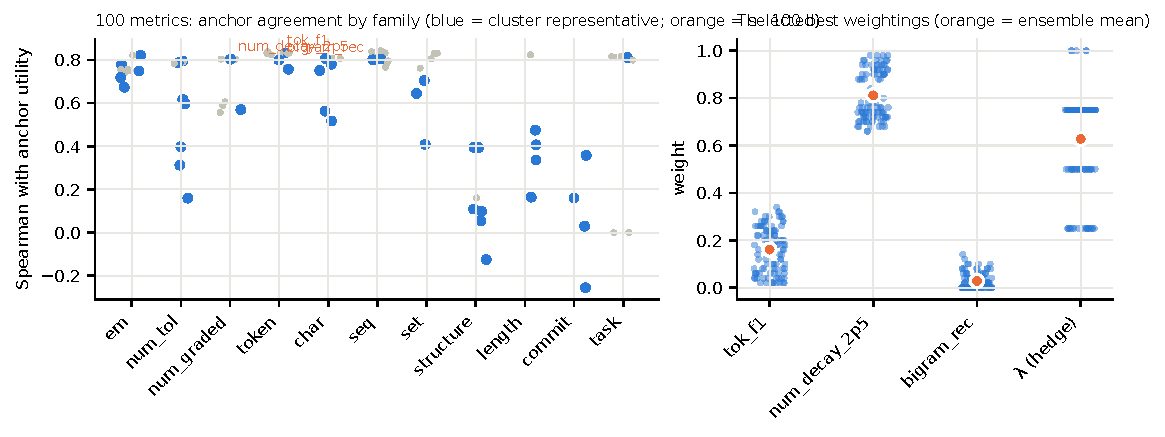
\includegraphics[width=0.95\textwidth]{figures/fig_selection.pdf}\caption{Left: anchor agreement of all 100 metrics by family (blue: cluster representatives; orange labels: selected). Right: the 100 best weightings and the hedge penalty.}\label{fig:sel}\end{figure*}
\begin{figure}[t]\centering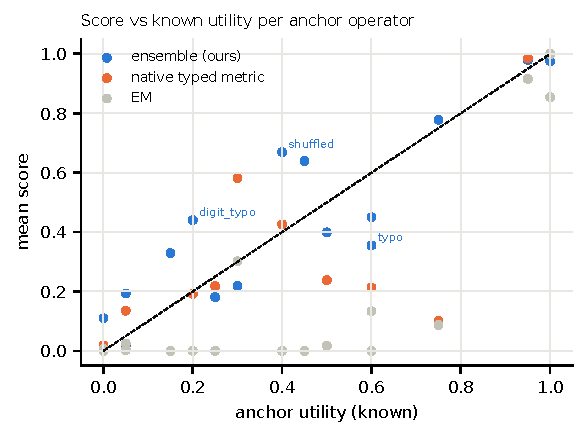
\includegraphics[width=0.85\linewidth]{figures/fig_probes.pdf}\caption{Mean score per anchor operator against its known utility.}\label{fig:probes}\end{figure}
\begin{figure*}[t]\centering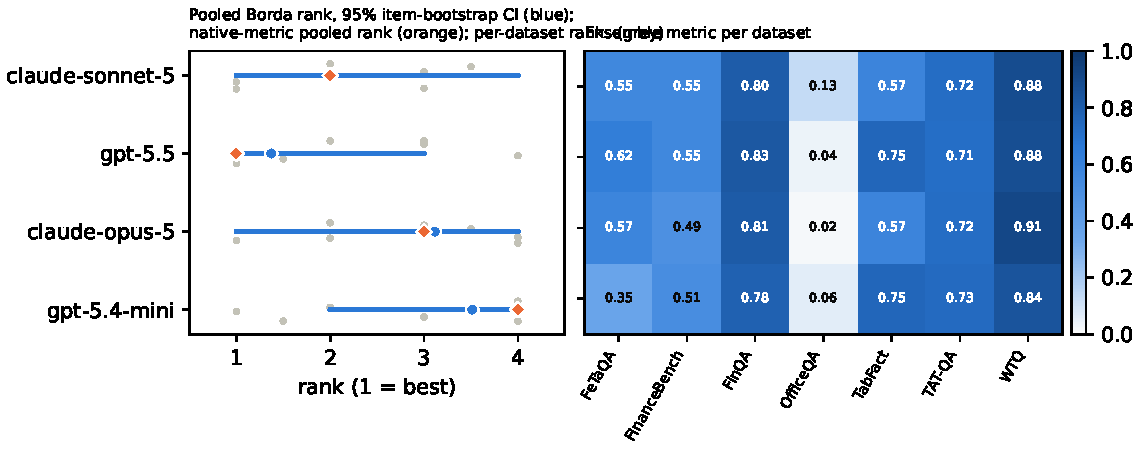
\includegraphics[width=0.95\textwidth]{figures/fig_leaderboard.pdf}\caption{Pooled Borda rank with item-bootstrap CI, native-metric pooled rank, per-dataset ranks; and the ensemble score per dataset.}\label{fig:lb}\end{figure*}
\begin{table*}[t]
\centering
\footnotesize
\caption{Forward selection on the anchor set (synthetic anchors (12813 answers, 20 operators)); 42 cluster representatives of 100 metrics were candidates.}
\label{tab:selected}

\begin{tabular}{rlllr}
\toprule
Step & Added metric & Family & LODO $\rho$ & Gain \\
\midrule
1 & tok\_f1 & token & 0.832 & +1.832 \\
2 & num\_decay\_2p5 & num\_graded & 0.879 & +0.047 \\
3 & bigram\_rec & token & 0.882 & +0.003 \\
4 & number\_set\_jaccard & set & 0.883 & +0.001 (stop) \\
\bottomrule
\end{tabular}

\end{table*}\begin{table*}[t]
\centering
\footnotesize
\caption{Single-metric baselines vs.\ the calibrated ensemble under the same objective (higher is better except JS and wrong$\to$, the mean score given to wrong or abstaining answers).}
\label{tab:baselines}

\begin{tabular}{lrrrrrr}
\toprule
Metric & $\rho_{anchor}$ & AUC & JS$_\times$ & wrong$\to$ & $\tau_{native}$ & $J$ \\
\midrule
native\_style\_metric & 0.830 & 0.918 & 0.038 & 0.004 & 0.924 & 0.913 \\
em\_norm & 0.848 & 0.952 & 0.031 & 0.002 & 0.629 & 0.882 \\
tok\_f1 & 0.852 & 0.956 & 0.066 & 0.006 & 0.544 & 0.860 \\
rouge\_l & 0.858 & 0.956 & 0.074 & 0.006 & 0.496 & 0.853 \\
num\_tol\_1 & 0.803 & 0.909 & 0.024 & 0.005 & 0.792 & 0.888 \\
uniform\_over\_selected\_no\_gate & 0.893 & 0.963 & 0.088 & 0.012 & 0.471 & 0.855 \\
ensemble\_top100 & 0.906 & 0.997 & 0.053 & 0.022 & 0.678 & 0.903 \\
\bottomrule
\end{tabular}

\end{table*}\begin{table*}[t]
\centering
\footnotesize
\caption{Mean score per anchor operator (all datasets). A calibrated metric tracks the utility column.}
\label{tab:probes}

\begin{tabular}{lrrrrrr}
\toprule
Operator & $u$ & $n$ & Ensemble & Native & EM & F1 \\
\midrule
identity & 1.00 & 1330 & 1.00 & 1.00 & 1.00 & 1.00 \\
verbose & 1.00 & 1330 & 1.00 & 1.00 & 1.00 & 1.00 \\
unit\_variant & 1.00 & 355 & 0.97 & 1.00 & 0.85 & 0.87 \\
tagged & 1.00 & 1330 & 1.00 & 1.00 & 1.00 & 1.00 \\
paraphrase & 0.95 & 1330 & 0.98 & 0.98 & 0.92 & 0.96 \\
near\_miss\_small & 0.75 & 355 & 0.78 & 0.10 & 0.09 & 0.09 \\
superset & 0.60 & 181 & 0.45 & 0.21 & 0.00 & 0.63 \\
typo & 0.60 & 120 & 0.35 & 0.13 & 0.13 & 0.57 \\
partial & 0.50 & 181 & 0.40 & 0.24 & 0.02 & 0.58 \\
near\_miss\_medium & 0.45 & 355 & 0.64 & 0.00 & 0.00 & 0.00 \\
shuffled & 0.40 & 61 & 0.67 & 0.43 & 0.00 & 1.00 \\
hedge & 0.30 & 1269 & 0.22 & 0.58 & 0.30 & 0.49 \\
list\_dump & 0.25 & 536 & 0.18 & 0.22 & 0.00 & 0.39 \\
digit\_typo & 0.20 & 355 & 0.44 & 0.19 & 0.00 & 0.00 \\
near\_miss\_large & 0.15 & 355 & 0.33 & 0.00 & 0.00 & 0.00 \\
sign\_flip & 0.05 & 355 & 0.02 & 0.00 & 0.00 & 0.01 \\
magnitude & 0.05 & 355 & 0.19 & 0.14 & 0.03 & 0.03 \\
flip & 0.00 & 794 & 0.00 & 0.00 & 0.00 & 0.00 \\
no\_answer & 0.00 & 1330 & 0.00 & 0.00 & 0.00 & 0.00 \\
wrong\_random & 0.00 & 536 & 0.11 & 0.02 & 0.01 & 0.03 \\
\bottomrule
\end{tabular}

\end{table*}\begin{table*}[t]
\centering
\footnotesize
\caption{Leave-one-dataset-out: selection and weights re-fitted without the held-out dataset, anchor Spearman on it.}
\label{tab:lodo}

\begin{tabular}{lrrr}
\toprule
Held-out & $\rho$ LODO & $\rho$ full & Selection (LODO) \\
\midrule
abt\_buy & 0.918 & 0.918 & tok\_f1, num\_decay\_2p5, bigram\_rec \\
amazon\_google & 0.919 & 0.919 & tok\_f1, num\_decay\_2p5, bigram\_rec \\
dblp\_scholar & 0.919 & 0.919 & tok\_f1, num\_decay\_2p5, bigram\_rec \\
fetaqa & 0.834 & 0.895 & tok\_f1, num\_decay\_2p5 \\
financebench & 0.868 & 0.867 & tok\_f1, num\_decay\_2p5 \\
finqa & 0.916 & 0.904 & tok\_f1, num\_decay\_2p5, bigram\_rec \\
hitab & 0.875 & 0.886 & tok\_f1, num\_decay\_2p5, chrf4, em\_raw \\
officeqa & 0.904 & 0.906 & tok\_f1, num\_decay\_2p5, prefix\_ratio \\
tab\_fact & 0.923 & 0.923 & tok\_f1, num\_decay\_2p5, bigram\_rec \\
tat\_qa & 0.879 & 0.881 & tok\_f1, num\_decay\_2p5, chrf4, em\_raw \\
tpcdi\_cells & 0.884 & 0.885 & tok\_f1, num\_decay\_2p5, prefix\_ratio \\
walmart\_amazon & 0.918 & 0.918 & tok\_f1, num\_decay\_2p5, bigram\_rec \\
wdc\_products & 0.920 & 0.920 & tok\_f1, num\_decay\_2p5, bigram\_rec \\
wikitablequestions & 0.853 & 0.853 & tok\_f1, num\_decay\_2p5, bigram\_rec \\
\bottomrule
\end{tabular}

\end{table*}\begin{table*}[t]
\centering
\small
\caption{Leaderboard under the ensemble metric: per-dataset means, difficulty-adjusted common score, pooled ranks, item-bootstrap CI, rank range across the 100 weightings, native-metric pooled rank.}
\label{tab:leaderboard}
\resizebox{\textwidth}{!}{%
\begin{tabular}{lrrrrrrrrrrrrr}
\toprule
Model & FeTaQA & FinanceBench & FinQA & OfficeQA & TabFact & TAT-QA & WTQ & $z$-mean & Borda & Kemeny & 95\% CI & over 100 $w$ & Native \\
\midrule
claude-sonnet-5 & 0.55 & 0.55 & 0.80 & 0.13 & 0.57 & 0.72 & 0.88 & +0.23 & 2 & 1 & [1, 4] & 1--2 & 2 \\
gpt-5.5 & 0.62 & 0.55 & 0.83 & 0.04 & 0.75 & 0.71 & 0.88 & +0.27 & 2 & 2 & [1, 3] & 1--2 & 1 \\
claude-opus-5 & 0.57 & 0.49 & 0.81 & 0.02 & 0.57 & 0.72 & 0.91 & -0.17 & 4 & 4 & [1, 4] & 3--4 & 3 \\
gpt-5.4-mini & 0.35 & 0.51 & 0.78 & 0.06 & 0.75 & 0.73 & 0.84 & -0.33 & 4 & 3 & [2, 4] & 3--4 & 4 \\
\bottomrule
\end{tabular}
}
\end{table*}

\section{Validation, limitations}\label{sec:val}
The anchor utility scale is a choice; we publish it, perturb it, and accept human labels in its place. The library is lexical (the semantic family is optional and off); the selected metrics show that on these tasks token F1 plus graded numeric error carry most of the information the library has. The objective's native-fidelity term deliberately keeps the composite close to what dataset authors report; a benchmark that prefers pure anchor agreement can set that coefficient to zero and will obtain a metric that is more severity-calibrated and less native-faithful. The model side is the binding constraint: four models and 40 items per dataset; \nPendingDatasets{} datasets are wired in with anchors and adapters and await predictions, and the model catalogue adds providers by adding keys.

\section{Conclusion}
A library of \nMetrics{} answer-level metrics, a synthetic anchor set of known utility, correlation deduplication with out-of-dataset forward selection, and a grid search whose \topK{} best weightings are averaged give one answer-level score that is calibrated to a stated severity scale, consistent across datasets, resistant to hedging, and close to native metrics, without ranking any model during calibration. It is the scoring rule of the v3 green agent and the basis of a difficulty-adjusted, uncertainty-aware leaderboard for data-matching agents.

\clearpage
\bibliographystyle{plainnat}
\bibliography{refs}
\end{document}
